% ----------------------------------------------------------
% Protocolos de comunicaçào
% ----------------------------------------------------------
\chapter[evolucao]{Evolução da comunicação entre aplicações}
%\addcontentsline{toc}{chapter}{Protocolos de Comunicação}
% ----------------------------------------------------------

Neste capítulo serão apresentados alguns dos principais protocolos para a comunicação entre aplicações. Serão conduzidas breves abordagens dos protocolos RPC e SOAP, que hoje vêm perdendo espaço no mercado, mas tiveram um papel muito importante para a evolução dos sistemas baseados em SOA. Em seguida, será mostrada uma descrição mais detalhada dos modelos de comunicação REST e GraphQL, uma vez que estes são os dois modelos a serem seguidos no estudo de caso.

Serão apresentados as principais características desses protocolos, como também as suas limitações. Nenhum dos protocolos pode ser descardado na hora de tomada de decisão sobre qual modelo utilizar para a comunicação entre clientes e serviços remotos ou APIs. Todos eles possuem limitações, porém cumprem bem o papel para que foram desenhados e é possível notar como eles evoluíram à medida que novas demandas se tornaram necessárias no desenvolvimento de \textit{software}.

\section{Remote Procedure Call}\label{sec:rpc}

Remote Procedure Call (RPC), ou Chamada de Procedimento Remoto, é um mecanismo em que uma aplicação solicita o serviço de uma outra aplicação que se encontra em um outro computador, geralmente conectados por uma rede. Uma RPC exige que uma aplicação X envie uma ou mais mensagens para outra aplicação Y a fim de invocar um procedimento da aplicação Y. A aplicação Y responde enviando uma ou mais mensagens de volta para a aplicação X. O termo RPC identifica todo o processo de comunicação entre as aplicações \cite{merrick2006xml}.

A RPC é similar ao modelo de  chamadas de procedimentos locais (IPC). Nas chamadas locais, a aplicação remetente envia argumentos para um procedimento localização no mesmo computador e transfere o controle da CPU para o procedimento. Logo após o término da execução, os resultados do procedimento são extraídos de uma localização compartilhada, e a aplicação remetente continua a sua execução \cite{rfc1831:rpc}. As chamadas remotas, por outro lado, aguardam a os resultados do procedimento diretamente da aplicação requisitada, como é ilustrado na figura \ref{fig:rpc}

\begin{figure}
\centering
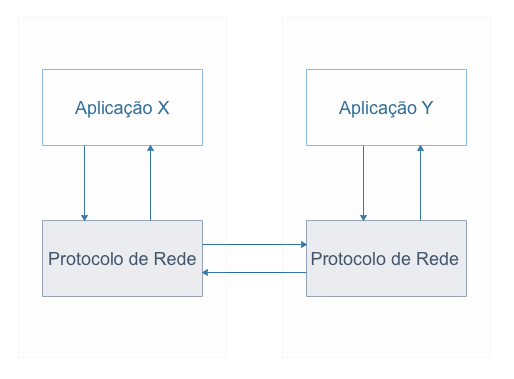
\includegraphics[width=0.7\textwidth]{figuras/rpc.png}
\caption{RPC fluxo de dados.}
\label{fig:rpc}
\end{figure}

Ainda, segundo a especificação da RPC \cite{rfc1831:rpc}, há alguns aspectos importantes em que as chamadas remotas se diferem das chamadas locais:

\begin{enumerate}[label=\alph*)]
\item \textbf{Tratamento de erros}: Falhas no servidor remoto ou da rede devem ser tratadas quando usando uma RPC.

\item \textbf{Variáveis globais}: Uma vez que o servidor não tem acesso ao espaço de endereço do cliente, argumentos ocultos não podem ser passados como variáveis globais. Todos os argumentos devem ser passados com a requisição.

\item \textbf{Desempenho}: Chamadas remotas geralmente operam uma ou mais ordens mais lentos do que chamadas de procedimentos locais.

\item \textbf{Autenticação}: Uma vez que as chamadas remotas podem ser transportadas através de redes insegurar, autenticação pode ser necessária.

\end{enumerate}

\subsection{Limitações}

Diferentes implementações de RPC são, geralmente, incompatíveis. Assim sendo, o uso de uma implementação específica, provavelmente resultará na dependência da implementação do fornecedor. Esse tipo de incompatibilidade entre diferentes implementações implica em um diverso número de funcionalidades, suportando inúmeros protocolos de rede e diferentes sistemas de arquivos.
%( https://www.eukhost.com/blog/webhosting/remote-procedure-call-rpc/ )

\citeonline{rpc-limitations} aponta diversas limitações técnicas e de desempenho encontradas em implementações de RPC's. Dentre estas limitações, se destacam:

\begin{enumerate}[label=\alph*)]

\item \textbf{Organização dos parâmetros}: para organizar os parâmetros, o cliente precisa conhecer a quantidade e a tipagem exata dos parâmetros. Como não existe um padrão bem definido, a estruturação dos parâmetros podem variar entre diferentes implementações.

\item \textbf{Falta de paralelismo}: com RPC, em um determinado momento, ou o servidor ou o cliente está ativo. Como cliente e servidor são co-rotinas, a prática de paralelismo presente em outros modelos de comunicação não é possível de ser implementada.

\item \textbf{Ferramentas de padronização}: as ferramentas padronizadas tornam-se muito mais difíceis de construir, devido ao grande número de implementações diferentes. Construir estas ferramentas geralmente requer o redesenho de convenções de tipo HTTP baseado sistema RPC escolhido, por consequencia da especialidade de cada sistema RPC.

\end{enumerate}

\section{Simple Object Access Protocol}\label{sec:soap}

Simple Object Access Protocol (SOAP) é um protocolo para troca de mensagens em ambientes descentralizados e distribuídos. \citeonline{soap2000} definem o SOAP como 
um protocolo baseado em XML que consiste em três partes: um envelope que defina um \textit{framework} para descrever o conteúdo das mensagens trafegadas e como processar este conteúdo, um conjunto de regras de codificação para expressar instâncias de tipos de dados definidos por uma aplicação, e uma convenção para representar chamadas remotas e suas respostas.

\citeonline{soap-tech-target} argumenta que o SOAP pode ser considerado parecido com as Chamadas de Procedimento Remoto (RPC), porém eliminando algumas das complexidades frequentemente encontradas nas implementações de RPCs. Utilizando o SOAP, é possível chamar serviços de outras aplicações que estão sendo executadas em qualquer \textit{hardware}, independente do sistemas operacional ou da linguagem de programação.

Embora a especificação do SOAP tenha evoluído para longe da necessidade de acessar objetos, como ocorre com as Chamadas de Procedimentos Remoto, existem ainda convenções para o encapsulamento e o envio de chamadas RPC utilizando uma representação uniforme de chamadas e repostas. Definindo um padrão para o mapeamento das chamadas RPC para SOAP, torna-se possível para infraestrutura traduzir as invocações de serviços em mensagens com o protocolo SOAP em tempo de execução, sem a necessidade de redesenhar todo o serviço Web presente na plataforma \cite{soap-microsoft}.

A figura \ref{fig:soap} ilustra como é realizada a troca de mensagens entre uma aplicação cliente e o servidor utilizando o SOAP. Como é possível observar, a aplicação cliente primeiramente serializa a mensagem e envia. Ao receber a requisição, o servidor precisa deserializar a mensagem, executar a consulta e serializar a mensagem de resposta. A aplicação cliente então, deserializa a resposta para poder manipulá-la.

\begin{figure}[htbp]
\centering
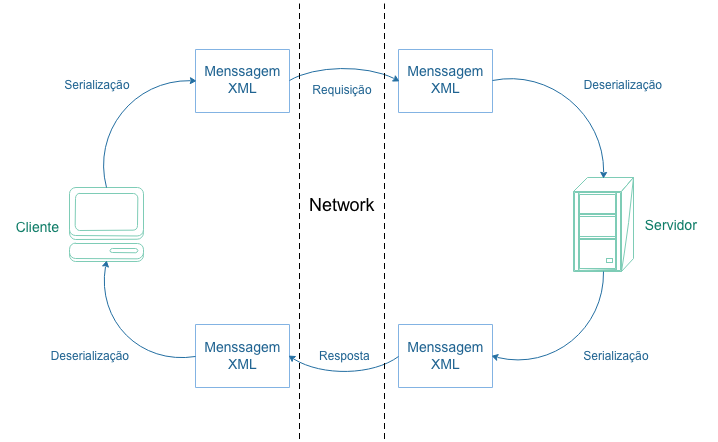
\includegraphics[width=1\textwidth]{figuras/soap.png}
\caption{SOAP fluxo de dados.}
\label{fig:soap}
\author{https://msdn.microsoft.com/en-us/library/x05s00wz(v=vs.80).aspx}
\end{figure}

\citeonline{soap-benefits} assinala que SOAP é um protocolo que define uma gramática XML especializada, que padroniza o formato das estruturas das mensagens. As mensagens são, por outro lado, o método fundamental de troca de informações entre os serviços Web e os seus consumidores. Ao utilizar XML para codificar mensagens,  o SOAP apresenta alguns benefícios:

\begin{enumerate}[label=\alph*)]

\item permite a comunicação entre sistemas protegidos por \textit{firewalls}, sem precisar abrir portas adicionais e, possivelmente, não seguras;

\item é mais fácil de entender e eliminar erros pois o formato XML pode ser mais facilmente lido e entendido;

\item as mensagens podem ser compreendidas por quase todas as plataformas de hardware, sistemas operacionais e linguagens de programação, uma vez que os dados do SOAP são estruturados usando XML;

\item pode ser usado, potencialmente, em combinação com vários protocolos de transporte de dados, como HTTP, SMTP e FTP;

\item O SOAP mapeia satisfatoriamente para o padrão de solicitação / resposta do HTTP;

\end{enumerate}

\subsection{Limitações}

\citeonline{soap-limitations} explica que tecnologias de metadados abertas, como o XML, podem fornecer um grande ganho de usabilidade, mas o sucesso dessas tecnologias exige que seu uso não degrade o desempenho de forma irracional. O XML é extremamente robusto, no entanto, o seu uso pode afetar negativamente o desempenho do SOAP nas seguintes áreas:

\begin{enumerate}[label=\alph*)]

    \item \textbf{Velocidade de codificação e decodificação}: a conversão de dados de binário para ASCII e vice-versa é o principal custo de desempenho do XML. O uso de um protocolo baseado em texto também impede a aplicação de otimizações disponíveis para protocolos binários quando a comunicação ocorre entre sistemas homogêneos;
    
    \item \textbf{Tamanho da mensagem}: para XML, um fator de expansão de 6-8 vezes em relação aos dados binários originais não é incomum. O tamanho da representação de dados do SOAP é tipicamente cerca de 10 vezes o tamanho da representação binária equivalente. Estes fatores resultam em maiores custos de transmissão de rede e latência aumentada;
    
\end{enumerate}

Como é possível notar, as maiores limitações encontradas na utilização do SOAP como modelo de comunicação estão relacionadas a estruturação usando XML. Embora esse formato padrão de mensagens tenha trazido vantagens em relação às tecnologias anteriores, ele também trouxe uma série de limitações conforme sua popularidade foi crescendo. A necessidade de buscar alternativas para superar esses problemas foi crescente, e novos formatos foram aparecendo, tendo como destaque o JSON.

\section{REpresentational State Transfer}\label{sec:rest}

REpresentational State Transfer (REST) é um \textit{design} de arquitetura baseado em um conjunto de princípios que descrevem como os recursos em rede são definidos e abordados. Estes princípios foram descritos pela primeira vez em 2000 por Roy Fielding, como parte de sua dissertação de doutorado \cite{rest-intro}.

\citeonline{programmableweb-rest-losing} assinala que a adoção do REST como o método predominante para construir APIs públicas tem ofuscado qualquer outra tecnologia ou abordagem nos últimos anos. Embora várias alternativas (principalmente SOAP) ainda estejam presentes no mercado, adeptos do modelo SOA, descrito da seção 2.4,  para construção de aplicações tomaram uma posição definitiva contra eles e optaram por REST como sua abordagem e JSON como seu formato de mensagem .

Segundo \citeonline{rest-book-intro:61}, REST é um padrão de operações de recursos que emergiu como a principal alternativa ao SOAP para o \textit{design} de serviços em aplicativos Web 2.0. Considerando que a abordagem tradicional baseada em SOAP para Web Services usa objetos remotos completos com invocação de método remoto e funcionalidade encapsulada, o REST trata apenas de estruturas de dados e da transferência de seu estado. A simplicidade do REST, juntamente com seu ajuste natural sobre o HTTP, contribuiu para o seu \textit{status} como um método de escolha para aplicativos da Web 2.0 expondo seus dados.

\subsection{Restrições}

As restrições do REST são regras desenhadas para estabelecer as características distintas da arquitetura REST. Cada restrição é uma decisão de projeto pré-determinada que pode ter impactos positivos e negativos. A intenção é que os aspectos positivos de cada restrição equilibrem os negativos para produzir uma arquitetura geral que se assemelhe à Web.

Uma arquitetura que elimina uma das restrições de \textbf{cliente/servidor}, \textbf{stateless}, \textbf{cache}, \textbf{interface uniforme}, \textbf{sistemas em camadas} ou \textbf{código por demanda}, geralmente é considerada como não mais conforme ao REST. Isso exige que as decisões sejam tomadas para entender os potenciais \textit{trade-offs} quando se desviam deliberadamente da aplicação de restrições REST. 

A primeira restrição estabelecida é a da arquitetura \textbf{cliente-servidor}, descrita na Seção 2.2. A separação de responsabilidades é o princípio por trás das restrições cliente-servidor. Ao separar as responsabilidades da interface do usuário com as responsabilidades de armazenamento de dados, é melhorada a portabilidade da interface do usuário em várias plataformas e a escalabilidade, simplificando os componentes do servidor. Talvez, o mais importante para a Web, no entanto, é que a separação permite que os componentes evoluam de forma independente, apoiando assim o requisito de escalabilidade da Internet de múltiplos domínios organizacionais \cite{rest-thesis}

Em seguida, foi adicionada ao REST uma restrição à interação cliente-servidor: a comunicação deve ser totalmente \textbf{stateless}, ou seja, independente de estado, de modo que cada solicitação do cliente deve conter todas as informações necessárias para entender o pedido e não pode tirar proveito de nenhum contexto armazenado no servidor. O estado da sessão é, portanto, mantido inteiramente no cliente \cite{rest-thesis}.

Essa restrição induz as propriedades de visibilidade, confiabilidade e escalabilidade. A visibilidade é melhorada porque um sistema de monitoramento não precisa olhar além de um único dado de solicitação para determinar a natureza completa da solicitação. A confiabilidade é melhorada porque facilita a tarefa de recuperação de falhas parciais. A escalabilidade é melhorada porque não precisar armazenar o estado das solicitações permite que o servidor rapidamente libere recursos, simplificando a implementação.

A restrição de \textbf{cache} foi criada para melhorar a eficiência da rede. Ela exige que os dados dentro de uma resposta a uma solicitação sejam rotulados de forma implícita ou explícita como cacheáveis ou não armazenáveis em cache. Se uma resposta for armazenada em cache, um cache do cliente terá o direito de reutilizar esses dados de resposta para solicitações equivalentes posteriores.

A vantagem de adicionar restrições de cache é que eles têm o potencial de eliminar parcial ou totalmente algumas interações, melhorar a eficiência, escalabilidade e desempenho percebido pelo usuário, reduzindo a latência média de uma série de interações. O \textit{trade-off}, no entanto, é que um cache pode diminuir a confiabilidade se os dados obsoletos dentro do cache diferirem significativamente dos dados que teriam sido obtidos se a solicitação fosse enviada diretamente para o servidor.

A característica central que distingue a arquitetura REST de outros estilos baseados em rede é a ênfase em uma \textbf{interface uniforme} entre os componentes. Ao aplicar o princípio de engenharia de software de especialização/generalização para a interface do componente, a arquitetura geral do sistema é simplificada e a visibilidade das interações é melhorada. As implementações são dissociadas dos serviços que eles fornecem, o que incentiva a evolução independente. O \textit{trade-off}, no entanto, é que uma interface uniforme degrada a eficiência, uma vez que a informação é transferida em uma forma padronizada e não específica para as necessidades de uma aplicação.

Para obter esta interface uniforme, são necessárias várias restrições arquitetônicas para orientar o comportamento dos componentes. REST é definido por quatro restrições de interface: identificação de recursos; manipulação de recursos através de representações; mensagens auto-descritivas; e, hipermídia como motor do estado da aplicação.

A fim de melhorar o comportamento dos requisitos de escalonamento, o REST também implementa restrições de \textbf{sistema em camadas}. O sistema em camadas permite que uma arquitetura seja composta de camadas hierárquicas ao restringir o comportamento dos componentes, de modo que cada componente não possa acessar além da camada imediata com a qual eles estão interagindo. Ao restringir o conhecimento do sistema a uma única camada, colocamos um limite na complexidade geral do sistema e promovemos a independência do componentes. As camadas podem ser usadas para encapsular serviços legados e para proteger novos serviços de clientes legados, simplificando componentes e movendo funcionalidades raramente usadas para um intermediário compartilhado. Os intermediários também podem ser usados para melhorar a escalabilidade do sistema ao permitir o balanceamento de carga de serviços em várias redes e processadores.

A principal desvantagem dos sistemas em camadas é que eles adicionam sobrecarga e latência ao processamento de dados, reduzindo o desempenho perceptível pelo usuário. Para um sistema baseado em rede que suporta restrições de cache, isso pode ser compensado pelos benefícios do armazenamento em cache compartilhado em intermediários.

A última restrição que o REST implementa é a restrição de \textbf{código por demanda}. O REST permite que a funcionalidade do cliente seja estendida baixando e executando o código na forma de \textit{applets} ou \textit{scripts}. Isso simplifica os clientes, reduzindo o número de recursos necessários para serem pré-implementados. Permitir que os recursos sejam baixados após a implantação melhora a extensibilidade do sistema, no entanto, reduz a visibilidade e, portanto, é apenas uma restrição opcional dentro do REST.

\subsection{Modelo de Maturidade de Richardson}

O Modelo de Maturidade de Richardson é um modelo criado por Leonard Richardson que descreve os requisitos necessários para o desenvolvimento de uma API REST bem estruturada e compatível com as restrições definidas pela arquitetura REST. Quanto melhor a API adere às restrições citadas na sessão anterior, melhor será pontuada. O modelo de Richardson, ilustrado na figura \ref{fig:rest-maturity-model}, descreve 4 níveis (0-3), onde o nível 3 designa uma API verdadeiramente \textit{RESTful}. Richardson usou três fatores para decidir a maturidade de uma API: URI (\textit{Uniform Resource Identifiers}), métodos HTTP e HATEOAS (Hypermedia). Quanto mais uma API emprega essas tecnologias, mais madura ela é categorizada.

\begin{figure}[htbp]
\centering
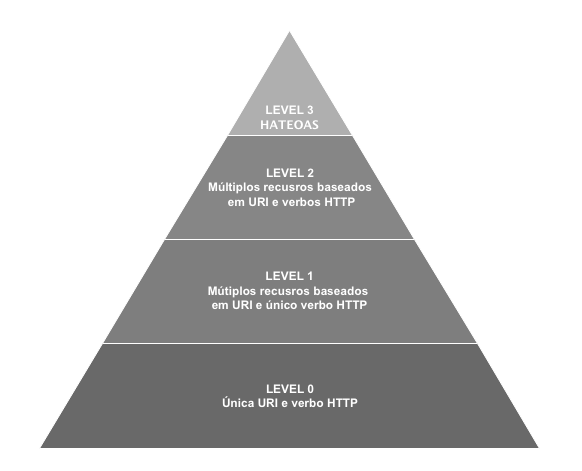
\includegraphics[width=0.93\textwidth]{figuras/modelo-maturidade.png}
\caption{Modelo de maturidade de Richardson.}
\label{fig:rest-maturity-model}
\end{figure}

Os níveis do modelo de maturidade de Richardson são:

\begin{enumerate}[label=\alph*)]

\item Nível 0: O ponto de partida para o modelo é usar HTTP como um sistema de transporte para iterações remotas, mas sem usar nenhum dos mecanismos da web. Essencialmente, o que está sendo feito é utilizar o HTTP como um mecanismo de tunelamento para seu próprio mecanismo de interação remota, geralmente com base em Chamadas de Procedimento Remotas. 

É como se estivesse sendo chamado funções, porém através do uso do HTTP. Todos os serviços são centralizados em um único \textit{endpoint}, ou seja, todas as solicitações são feitas em uma única URI.

\item Nível 1: Quando uma API faz a distinção entre recursos diferentes, pode se considerar que atingiu o nível 1. Esse nível usa vários URIs, em que cada URI é o ponto de entrada para um recurso específico. Ainda assim, esse nível usa apenas um único método, como o POST.

\item Nível 2: Esse nível indica que a API deve usar as propriedades do protocolo para lidar com escalabilidade e falhas. Não é recomendado que se use um único método POST para todas as chamadas, mas faça uso do GET quando estiver solicitando recursos e use o método DELETE quando desejar excluir recursos. Além disso, o uso dos códigos de resposta do protocolo de aplicação também é recomendado. Não deve ser usado, por exemplo, o código 200 (OK) quando algo der errado.

\item Nível 3: O nível três de maturidade faz uso de todos os três fatores, isto é, URIs, métodos HTTP e HATEOAS. Esse é o nível em que a maioria das APIs menos implementam e pois não seguem o princípio de HATEOAS.

\end{enumerate}

HATEOAS (Hypermedia as the Engine of Application State) é uma abordagem para a construção de serviços REST, em que o cliente pode descobrir dinamicamente as ações disponíveis em tempo de execução. Todo cliente deve exigir uma URI inicial e um conjunto de tipos de mídia padronizados para começar a troca de mensagens. Uma vez que carregou o URI inicial, todas as futuras transições de estado da aplicação serão conduzidas pelo cliente selecionando as escolhas fornecidas pelo servidor.

Não seguir essa abordagem não é necessariamente ruim. Há alguns bons argumentos a serem feitos a favor e contra a utilização de HATEOAS. Enquanto, por um lado, torna as APIs fáceis de descobrir e usar, por outro, eleva o tempo e o esforço de desenvolvimento das aplicações.

\subsection{Limitações}

Contudo, com a evolução e o aumento da complexidade das APIs, a comunicação via o protocolo REST vem se mostrando muitas vezes inviável pois sua implementação trás como consequências alguns problemas estruturais como:

\begin{enumerate}[label=\alph*)]

\item a necessidade de executar múltiplas requisições entre o cliente e o servidor a fim de obter objetos complexos e com atributos aninhados  Para aplicações móveis operando em condições variáveis de rede, essas múltiplas viagens de ida e volta são indesejáveis, pois geram atrasos e maior tráfego na rede \cite{graphQl-overview};

\item a prática de \textit{over-fetching}, ou seja, quando o cliente busca alguma informação do servidor e a resposta contém mais informação que o cliente precisa. Esse tipo de problema acarreta no uso desnecessário de recursos de comunicação  \cite{efficient-data-communication};

\item o versionamento da API, que ocorre quando há alterações significativas na API, sujeitas a quebra de código nos clientes consumidores. Essa prática pode ser extremamente penosa se a API é usada por uma grande massa de clientes que não são facilmente atualizados \cite{api-versioning};

\end{enumerate}

\section{Arquiteturas baseadas em JSON/Graphs}\label{sec:graph}

Recentemente, um novo design de arquitetura vem ganhando espaço, preenchendo algumas lacunas que arquiteturas anteriores deixaram. Lideradas pelo Facebook com seu GraphQL e Netflix com o Falcor, esta nova arquitetura da um passo para trás comparando-se ao REST, atingindo apenas o nivel 0 no Modelo de Maturidade de Richardson. 

Os principais problemas que essa arquitetura ajuda a resolver são: 

\begin{enumerate}[label=\alph*)]

\item a dependência das aplicações cliente nos servidores, eliminando a necessidade do servidor de ter que manipular as informações ou o tamanho da resposta; 

\item a necessidade de executar diversas requisições para acessar os dados exigidos por uma \textit{view};

\item melhorar a experiência de desenvolvimento \textit{frontend}, pois existe uma relação próxima entre os dados necessários à interface da aplicação e a forma como um desenvolvedor pode expressar uma descrição desses dados para a API. 

\end{enumerate}

O presente trabalho irá apenas focar no GraphQL como representante das arquiteturas baseadas em JSON/Graph.

GraphQL é uma linguagem de consulta, criada pelo Facebook em 2012, que fornece uma interface comum entre o cliente e o servidor para manipulação e busca de dados. GraphQL utiliza de um sistemas chamado \textit{cliente-specified queries}, onde o formato de resposta de uma requisição é definida pelo cliente. \citeonline{graphQl-overview} afirma que uma vez que a estrutura de dados não é codificada, como nas APIs tradicionais, a consulta de dados do servidor se torna mais eficiente para o cliente.

Consultas utilizando GraphQL sempre retornam apenas o que foi pré definido pela requisição, fazendo suas respostas sempre serem previsíveis. As consultas com GraphQL acessam não apenas as propriedades de um único recurso, mas também seguem as referências entre eles. Enquanto as APIs REST típicas exigem o carregamento de múltiplas URLs, as APIs GraphQL obtêm todos os dados que precisam em uma única requisição.

Adicionar novos campos ou tipos à uma API GraphQL não afeta nenhuma consulta ou funcionalidade já existente. Campos não mais utilizados podem ser obsoletos e ocultos de ferramentas de mapeamento. Ao usar uma única versão em evolução, as APIs GraphQL dão às aplicações acesso contínuo a novos recursos e encorajam um código de servidor mais limpo e mais sustentável.

\subsection{Operações}

Existem três tipos de operações modeláveis com GraphQL:

\begin{enumerate}[label=\alph*)]
\item \textbf{Query}: Uma consulta de somente leitura;
\item \textbf{Mutation}: Uma escrita seguida por uma consulta;
\item \textbf{Subscription}: Uma requisição de longa duração que obtém dados em resposta a eventos disparados pelo servidor;
\end{enumerate}

Uma Query em GraphQL é uma maneira de obter dados de uma maneira somente de leitura em uma API GraphQL. De uma maneira geral, GraphQL se baseia em consultar campos específicos em objetos. Isso significa que a consulta tem exatamente o mesmo formato que a resposta. Isso é essencial para GraphQL porque a resposta é sempre previsível, e o servidor sabe exatamente quais os campos que o cliente está pedindo.

Como GraphQL não se limita apenas em consultas de dados, as APIs também podem implementar operações para criar, atualizar e destruir dados. Para esses tipos de operações, o GraphQL usa o termo Mutations. As Mutations são uma maneira de alterar dados em seu servidor. É importante notar que as \textit{mutations} consistem em uma alteração seguida de uma busca do dado que acabou de ser alterado, tudo em uma única operação.

Os aplicativos em tempo real precisam de uma maneira de enviar dados do servidor. As \textit{subscriptions} permitem que aplicações publiquem eventos em tempo real através de um servidor de assinaturas GraphQL. Com o modelo de subscriptions baseado em eventos no GraphQL - muito parecido com as \textit{queries} e \textit{mutations} - um cliente pode dizer ao servidor exatamente quais dados devem ser enviados e como esses dados devem ser encontrados. Isso leva a menos eventos rastreados no servidor e notificados para o cliente.

\subsection{Schemas e Tipos}

%https://facebook.github.io/graphql

O sistema de tipos do GraphQL descreve as capacidades de um servidor GraphQL e é usado para determinar se uma consulta é válida. O sistema de tipos também descreve os formatos de entrada de variáveis de consulta para determinar se os valores fornecidos em tempo de execução são válidos. As capacidades do servidor GraphQL são referidas como \textit{schema} do servidor. Um \textit{schema} é definido baseado nos tipos que ele suporta.

Cada servidor GraphQL define um conjunto de tipos que descrevem completamente o conjunto de dados possíveis que você pode consultar nesse servidor. Então, quando as consultas chegam, elas são validadas e executadas contra os \textit{schemas}. O \textit{schema} descreverá quais campos o servidor pode responder e quais tipos de objetos estarão contidos nas respostas. A informação de tipo é muito importante para o GraphQL e o cliente pode assumir de forma segura que o servidor retornará tipos consistentes de objetos para o mesmo campo.

A unidade fundamental de qualquer \textit{schema} GraphQL é o tipo. Existem oito formatos de tipos suportados no GraphQL. O tipo mais básico é o \textit{\textbf{Scalar}}. Um campo do tipo \textit{Scalar} representa um valor primitivo, como uma \textit{string} ou um número inteiro. Muitas vezes, as respostas possíveis para um campo  do tipo \textit{Scalar} são enumeráveis. O GraphQL oferece um tipo \textit{\textbf{Enum}} nesses casos, onde o tipo especifica o espaço de respostas válidas. Campos do tipo \textit{\textbf{Object}} definem um conjunto de campos, onde cada campo é outro formato, permitindo a definição de hierarquias de tipos arbitrários. O GraphQL suporta dois tipos abstratos:  \textit{\textbf{Interfaces}} e  \textit{\textbf{Unions}}.

Todos os tipos até agora são considerados nulos e singulares, por exemplo,  uma \textit{string} retorna um valor nulo ou singular. O sistema de tipo pode querer definir que ele retorna uma lista de outros tipos. O tipo \textit{\textbf{List}} é fornecido por esse motivo e envolve outro tipo. Da mesma forma, o tipo \textit{\textbf{Non-Null}} envolve outro tipo e indica que o resultado nunca será nulo.

Finalmente, muitas vezes é útil fornecer estruturas complexas como entradas para consultas GraphQL; o tipo \textit{\textbf{Input Object}} permite que o \textit{schema} defina exatamente quais dados são esperados do cliente nessas consultas.

\subsection{Caching}

De acordo com \citeonline{graph-cache}, consultas de dados através da internet podem ser lentas e custosas, e por esse motivo, a capacidade de armazenar em cache e reutilizar os recursos obtidos anteriormente é um aspecto crítico da otimização para o desempenho.

\begin{figure}[htbp]
\centering
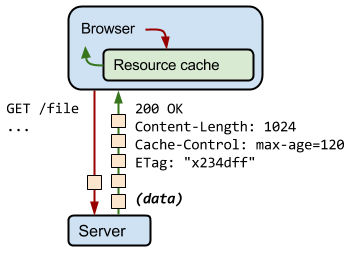
\includegraphics[width=0.5\textwidth]{figuras/cache-http.png}
\caption{HTTP Caching.}
\legend{Fonte: \citeonline{graph-cache}}
\label{fig:cache-http}
\end{figure}

Em uma API baseada em \textit{end-points}, os clientes podem usar o armazenamento em cache do protocolo HTTP, ilustrado na figura \ref{fig:cache-http} para evitar buscas desnecessárias identificando quando dois recursos são iguais. A URL nessas APIs é o identificador globalmente exclusivo que o cliente pode aproveitar para criar um cache. No GraphQL, porém, não existe uma primitiva semelhante a uma URL que forneça esse identificador globalmente exclusivo para um determinado objeto. Entretanto, existem várias práticas que podem ser aplicadas a um servidor GraphQL para atingir o mesmo objetivo.

Um padrão possível para isso é reservar um campo, como \textup{id}, para ser o identificador globalmente exclusivo. Da mesma forma que os URLs de uma API baseada em recursos fornecem uma chave globalmente exclusiva, o campo \textup{id} neste sistema fornece uma chave globalmente única. Outra abordagem possível funcionaria de forma semelhante ao padrão usada nas APIs baseadas em \textit{end-points}. O texto da consulta em si pode ser usado como identificador globalmente exclusivo. 

\subsection{Limitações}

Segundo aponta \citeonline{graph-limitation}, uma ameaça importante que o GraphQL \emph{facilita} são os ataques de negação de serviço. Um servidor GraphQL pode ser atacado com consultas excessivamente complexas que irão consumir todos os recursos do servidor. Esse tipo de ataque não é específico do GraphQL, mas é preciso um cuidado redobrado para evitá-los.

Há, entretanto, alguns procedimento que, se implementados, podem mitigar a ameaça de negação de serviço. É possível fazer uma análise de custos na consulta com antecedência e impor \emph{um certo tipo} de limites na quantidade de dados que uma requisição pode consumir. Também é possível implementar um tempo limite para que requisições que levam muito tempo para serem resolvidas, sejam excluídas da fila de execução .

%https://arxiv.org/pdf/1701.00626.pdf

